\documentclass[11pt]{amsart}
\usepackage{geometry}                % See geometry.pdf to learn the layout options. There are lots.
\geometry{letterpaper}                   % ... or a4paper or a5paper or ... 
%\geometry{landscape}                % Activate for for rotated page geometry
%\usepackage[parfill]{parskip}    % Activate to begin paragraphs with an empty line rather than an indent
\usepackage{graphicx}
\usepackage{amssymb}
\usepackage{epstopdf}
\DeclareGraphicsRule{.tif}{png}{.png}{`convert #1 `dirname #1`/`basename #1 .tif`.png}

\title{On Bayesian g-Computation and Instrumental Variables}
\author{P. Gustafson  and H. Campbell}
%\date{}                                           % Activate to display a given date or no date

\begin{document}
\maketitle
\section{Introduction}
\nocite{*}
After a marked change in treatment strategy, there is an obvious desire to infer the benefit of this change, often in terms of longer-term outcomes than can be assessed in clinical trials.
Thus there is a need to use observational data, but this is typically accompanied by concern about confounding by indication - if patients start on the new therapy because they aren't doing well, straight-up comparisons of ever versus never treated patients are not fair.   One strategy is to apply modern causal inference tools that can appropriately deal with this.  Another, seemingly cruder strategy, would involve treating calendar period of reaching eligibility for treatment as an instrumental variable.   Each approach involves very strong assumptions, though interestingly they are different assumptions, one not stronger than the other.  So we want to compare, at least in terms of power to detect treatment efficacy in the first instance.

\begin{figure}[h]
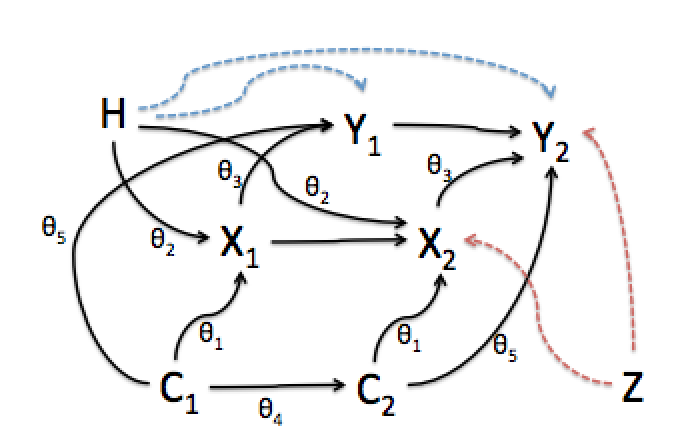
\includegraphics[width=11cm]{pic1.png}
\caption{Okay}
\centering
\end{figure}

\begin{figure}[h]
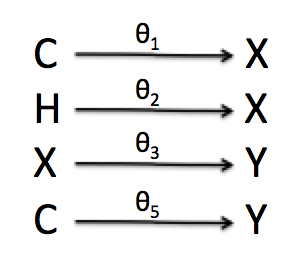
\includegraphics[width=6cm]{pic2.png}
\caption{Okay}
\centering
\end{figure}


%\begin{equation}
%Pr(H=h_{i}) \cdot Pr(C_{1}=c_{i} | H=h_{i}) \cdot  Pr(C_{2}=c_{i} | H=h_{i}, C_{1}=c_{i})
%\end{equation}


 \section{Methods}
 
- run down of the simple sandbox of two time-points, everything binary 
	- g-computation (perhaps motivated several different ways)
	- IV idea

Comparison in a focussed scenario
-	confounding by indication present (C encourages treatment start)
-	different possible forms of treatment effect (through C and/or around C)
-	both sets of assumptions met

Comparison across a broad range of scenarios

-	set up distribution giving rise to a wide array of states of the world
-	look for patterns, e.g., is the power of the g-computation driven only by theta11-theta00, or are there other important factors
    
Violations of assumptions

-	any defensible sense of one procedure being more robust than the other
-	how quickly is power lost as we relax assumptions


 \section{Application}

I don?t know whether we?d find a good ?real-data? example, but we could address the question of how much data we would need (how many subjects, over how long a time period) in order to say something useful about the efficacy of beta-interferon for MS in terms of long-term disability.

Random citation \cite{saarela2015bayesian} embeddeed in text.



 \section{Discussion}
\newpage

\bibliography{gcomp_refs} 
\bibliographystyle{ieeetr}


\end{document}  